\documentclass[output=paper]{LSP/langsci}  
\author{Ivana Škevin\affiliation{University of Zadar}} 
\title{Dialect levelling and changes in semiotic space}
\abstract{The Betina variety is a local Čakavian-Croatian variety spoken on the island of Murter in central Dalmatia. The influence of Romance has left visible traces on the island’s vocabulary, just as it has in many other Čakavian varieties of the Eastern Adriatic coast. The Betina variety, through contact with other, more dominant dialectal varieties or the Croatian standard variety, and as a consequence of language accommodation, is losing many of its most salient, mostly Romance, characteristics, a process that is leading to a loss of local distinctiveness. This paper proposes a semiotic approach to the problem of dialect levelling and assumes that it occurs not only because of language accommodation, but also as a consequence of the alteration and transformation of the culture and of the ways of life referred to as semiotic spaces. Since a language or dialect can function only in interaction with its semiotic space, its change leads to language change. The analysis was conducted on a selected lexical corpus of Romance origin and involved interviews with young speakers living in Betina. The results of this study are expected to confirm that in Betina, particularly in the vocabulary of young speakers, Romance elements are disappearing as a consequence of the disappearance of human practices and of utilitarian and sociocultural objects that once had an important role and which used to create very particular and distinctive semiotic spaces.

}

\maketitle 
\begin{document}
 

% {\centering \\
% \centering \\}
 

\section{Introduction}
Over the centuries, our needs as humans change; the objects we use and the activities we engage in disappear and get (re)constructed; and our way of life changes together with the ways in which we make a living, eat, get our food, and dress. All these components of life are intimately connected. One cannot exist without the other; they all create meaning and are generally considered to be secondary modeling systems. These systems are secondary in relation to the primary system of language because, like all semiotic systems, they are constructed on the model of language \citep[viii]{lotman_culture_2009}. It is possible to suggest that, in reality, clear and functionally mono-semantic systems do not exist in isolation. No one system, in fact, is effective when taken individually. The starting point of this research is Lotman's assumption that, without the semiosphere — that is, the semiotic space of the culture in question — language not only does not function but does not exist \citep[218--219]{lotman_semiosphere_1985}. Accordingly, the current article deals with linguistic and semiological signs. \citet[41]{barthes_elements_1968} claims that a semiological sign, like its linguistic model, comprises a signifier and a signified, but that it differs from a linguistic sign at the level of the substance of its expression, the essence of which is not to signify but to have function and utility in everyday use. 

\section{Linguistic, Historical and Socioeconomic Background}
The Croatian language has three main groups of dialects: \textit{Kajkavian, Čakavian,} and \textit{Štokavian.} Their names derive from the form of the interrogative pronoun (\textit{kaj, ča, }and \textit{što }‘what’) used in each dialect\textit{.} Standard Croatian is based on Štokavian. The dialects of the Čakavian group, one of which is the subject of this study, are spoken along the East Adriatic Coast. Čakavian has many local varieties, which vary in terms of accentuation, morpho-syntax, or lexicon. The local dialect spoken in Betina, a village on the island of Murter in central Dalmatia, belongs to the group of Southern Čakavian Ikavian varieties. One of its main characteristics, which it shares with most other Čakavian varieties, is that a great majority of its technical vocabulary in specific fields is of Romance origin.\footnote{Research undertaken in 2008, 2009, and 2010 has revealed that in the Betina dialect loanwords of Romance origin account for 61.96\% of fishing terminology, 65.12\% of maritime terminology, 29.41\% of wine terminology, 36.73\% of olive cultivation terminology, 57.14\% of barrel-making terminology, and finally, 61.54\% of agricultural terminology (tools and maintainance of arable land) \citep[254--255]{skevin_etimoloska_2010}.} Romance lexical elements originate from the now extinct Dalmatic languages as well as from old dialectal varieties of Italian that functioned as proper languages in past centuries (Venetian and Triestine, as well as Italian).\footnote{ Dalmatic languages were spoken on the eastern Adriatic coast from the 9th until the 13th century in central Dalmatia, until the 16th century in Dubrovnik, and until the 19th century on the northeastern Adriatic island of Krk. Venetian, very often referred to as Colonial Venetian, was the \textit{lingua franca }of the eastern Adriatic for many centuries. Its influence was the strongest between the early 16th and the late 18th century. After the fall of the Serenissima, Trieste became the centre from which spread a new Venetian variety – Triestine. At the beginning of the 20th century, especially during the First World War, began the expansion of the Italian language, which lasted until the Second World War.} Previous research and etymological analysis have shown that a great majority of the loanwords used in the Čakavian variety of Betina are of Venetian origin \citep{filipi_betinska_1997,skevin_etimoloska_2010}. Croatians borrowed from the Venetians the objects and the corresponding words they needed to understand and sail the sea, to build boats, and to cultivate wine and olives, thus creating their semiotic space. The borrowed words naming these everyday needs and ways of life became integral lexical forms and structures of the Čakavian-Croatian Adriatic varieties.

This research concentrates on the case of Betina, though we claim that in fact it reflects the dialectal situation of many other small local varieties of central Dalmatia. Although situated on an island, we cannot define Betina as an isolated island community, but as part of the Adriatic coast, since it is connected to the mainland by a bridge. The bridge makes it easily accessible and was one of the key factors for the community’s rather early development of tourism, which started in the 1960s \citep[138]{kulusic_murterski_1984}. The main economic activities in Betina in 1971 were agriculture, fishing, and the building of traditional wooden boats. Agriculture was the main primary activity of most villagers and a source of income because the inhabitants produced fruits and vegetables, olive oil, and wine for sale and for their own needs, whereas fishing served mostly to satisfy the dietary needs of every household. Before the Second World War, there were numerous small private shipyards, which in 1948 were merged into one \citep[21]{filipi_betinska_1997}.\footnote{In 1926 there were one large and nine small shipyards. Betina’s shipyards covered a total of 11,200 square meters, which was greater than the total surface area of shipyards in the rest of Northern Dalmatia, which was 10,330 square meters. In 1930, ten private shipyards were registered in Betina. The 1930s marked the beginning of a crisis in the sector of traditional wooden boat building \citep[19]{filipi_betinska_1997}.} In 2014, besides the main shipyard, there are two smaller ones. \tabref{tab:1} represents the percentage of the population of Betina working in different economic sectors in the years 1971 and 2001 \citep[21]{skracic_otok_2010}.

\begin{table}
\begin{tabular}{lll} 
% & {\bfseries YEAR} &
\lsptoprule
ECONOMIC SECTOR & 1971 & 2001\\
\midrule
{\scshape agriculture, fishing} & 38\% & 21\%\\
{\scshape Industry (wooden boat building)} & 30\% & 18\%\\
{\scshape Service (tourism)} & 9\% & 45\%\\
{\scshape public sector} & 0\% & 6\%\\
{\scshape people working abroad} & 20\% & 8\%\\
\lspbottomrule
\end{tabular}
\caption{Percentage of the population of Betina employed in different economic sectors in the years 1971 and 2001 \citep{skracic_otok_2010}.}
\label{tab:1}
\end{table}

There was a noticeable decline in the primary (agriculture and fishing) and secondary (industrial) sectors, as well as an increase of 36\% in the tertiary sector (tourism), during the period between 1971 and 2001. The population’s reorientation to the tertiary sector of the economy led to the abandonment of arable land, excessive urbanization, and the degradation of the natural and cultural identity of the island. As a consequence of these social changes, the dialectal identity of Betina’s population changed as well.

\begin{table}
\begin{tabular}{llll}
\lsptoprule
year & 1971 & 2001 & 2011\\
\midrule
no.  of inhabitants & 988 & 774 & 697\\
\lspbottomrule
\end{tabular}
\caption{Population change in Betina from 1971 to 2011 (\citealt[15]{skracic_otok_2010} and \citealt{drzavni_zavod_za_statistiku_republike_hrvatske_1})}
\label{tab:2}
\end{table}

Besides that, as \tabref{tab:2} shows, the population of Betina has dropped by almost 30\% in the last four decades.

\section{Methodology and Hypothesis}
This study focused on a selected lexical corpus of mostly Romance origin, and it involved interviews conducted by the present author (an in-group researcher) with seven young adult speakers (ranging in age from 22 to 40) living in the village of Betina on the island of Murter in central Dalmatia. The questionnaire consisted of 70 lexemes. This corpus is a small subset of a much wider corpus collected and registered during interviews with older speakers between the ages of 50 and 90 conducted in Betina during the years 2008, 2009 and 2010 \citep{skevin_etimoloska_2010}. The lexemes were chosen so that they would belong to different spheres of life: household, maritime and fishing, viticulture and olive cultivation, folklore and church. These are (or at least used to be) very important aspects of the life and culture of Betina. 

This study concerns intergenerational variation mainly in connection with the social context of variation and change and is expected to confirm a hypothesis that in Betina, particularly in the vocabulary of young speakers, the Romance elements are disappearing for two reasons: as a consequence of the local variety’s convergence toward the Supra-regional Dalmatian Dialect (SRDD) and toward Standard Croatian (SC) and as a consequence of the disappearance of human practices and utilitarian objects that once had an important role and which used to create very specific and distinctive semiotic spaces. Since a language or a dialect can function only in interaction with its semiotic space, changes in that space should lead to language change. 

\section{Sociolinguistic and Semiotic Approach to Dialect levelling}
The results presented in \tabref{tab:3} suggest that there is a pattern which determines the speakers’ knowledge and usage of the variants. The least-known variants (numbers 1-34, with the exception of the variant \textit{gvantijera }‘a tray’) refer to referents or concepts that have lost importance in the daily life of Betina (e.g., \textit{batusić/batusigaj }'an inside, hollowed-out part at the bottom of a well where water gets trapped'\textit{, gaštaldo }'a person who helps the priest in the church'\textit{, štiva }‘the interior part of a boat under the bow') or whose referent is not in use any more (e.g., \textit{bujo(l) }‘a wooden bucket held on traditional Dalmatian boats, used to remove sea water’\textit{, burača }‘a leather sack for keeping wine’\textit{, dumplir }‘a wooden candlestick carried during a funeral’). The second group of variants (from number 35 onwards), which the users know better and use more often, mostly, but not always, name referents or concepts whose function in everyday life has not changed. These include words that, for example, refer to household objects (such as \textit{prsura }‘a frying pan’\textit{ kočeta }a bed’\textit{, škabelin }‘a nightstand’\textit{, čikara }‘a mug’). In this second group, though, there are also variants that name objects whose function in the daily life of Betina has changed. For example, variants like \textit{škohuni }‘type of shoes worn during work in the fields’\textit{, bukara }‘a large wooden wine cup’\textit{, brganja }‘a type of a fishing tool’\textit{, kajin }‘a round metal vessel used for washing clothes’\textit{, pičona }‘a metal cup with a handle’ name objects that are out of use, whereas \textit{burtižati }‘to sail into the wind’, \textit{paj} ‘a scoop used for throwing sea-water out of a boat’ and \textit{rehud} ‘a sudden, brief gust of wind’ name referents or concepts whose role in the daily life of Betina has become less prominent\textit{. }These results suggest that, contrary to the anticipated hypothesis, a change in the semiotic space does not always lead to dialect change. They also show that in some cases there is a divide between familiarity with a variant and its actual use. For example, all speakers know the meaning of the variants \textit{bruncin }and \textit{kočeta}. However, all of them also declare that they do not use them in any communication situation. In this article we propose two approaches to the challenges of dialect levelling: a sociolinguistic approach, which concerns changes in to the use of variants in different social contexts, and a semiotic approach, which concerns change in the way of life of the community and the transformation of its semiotic spaces.


\begin{table}
\caption{Vitality of lexical variants}
\label{tab:3}

\resizebox{\textwidth}{!}{
\begin{tabular}{lp{.2\textwidth}p{.5\textwidth}lrlr}
\lsptoprule
%{\bfseries no.} 
& {\bfseries lexeme} & {\bfseries meaning} & \multicolumn{2}{p{.2\textwidth}}{\bfseries informants who knew the word's meaning} & \multicolumn{2}{p{.2\textwidth}}{\bfseries informants who use the word}\\
& & & n & \% & n & \%\\
\midrule

{\bfseries 1} & {\itshape brganjaš} & 
'the wind that favors bottom trawling with a \textit{brganja'} & 0 & 0 & 0 & 0\\

{\bfseries 2} & {\itshape bujo(l)} & 
'a wooden bucket held/kept on traditional Dalmatian boats, used to remove sea water' & 0 & 0 & 0 & 0\\

{\bfseries 3} & {\itshape goče} & 'a part of a fishing net' & 0 & 0 & 0 & 0\\

{\bfseries 4} & {\itshape koslata} & 'a type of a barrel vertically placed on a trailer' & 0 & 0 & 0 & 0\\

{\bfseries 5} & {\itshape tinac} & 'a type of a vessel similar to \textit{mastač,} but smaller and without handles' & 0 & 0 & 0 & 0\\

{\bfseries 6} & {\itshape batusić / batusigaj} & 'an inside, hollowed-out part at the bottom of a well where water gets trapped, so there's water even when the well is almost empty' & 1 & 14.28 & 0 & 0\\

{\bfseries 7} & {\itshape burača} & 'a leather sack for keeping wine' & 1 & 14.28 & 0 & 0\\

{\bfseries 8} & {\itshape dumplir} & 'a wooden candlestick carried during a funeral' & 1 & 14.28 & 0 & 0\\

{\bfseries 9} & {\itshape gaštaldo} & 'a person who helps the priest in the church' & 1 & 14.28 & 1 & 14.28\\

{\bfseries 10} & {\itshape komoštra} & 'one of the metal rings of the chain used to hang pots over the fire' & 1 & 14.28 & 0 & 0\\

{\bfseries 11} & {\itshape murtar} & 'a stone container used for storing olive oil. It comes in different sizes' & 1 & 14.28 & 1 & 14.28\\

{\bfseries 12} & {\itshape taraban} & 'a church custom that consists in making lots of noise by striking an object with one's hands or with a stick' & 1 & 14.28 & 0 & 0\\

{\bfseries 13} & {\itshape štiva} & ‘the interior part of a boat under the bow' & 2 & 28.57 & 2 & 28.57\\

{\bfseries 14} & {\itshape butarga} & 'fish eggs' & 2 & 28.57 & 1 & 14.28\\

{\bfseries 15} & {\itshape baraškada} & 'a small sea storm' & 2 & 28.57 & 1 & 14.28\\

{\bfseries 16} & {\itshape brenda} & 'a flat wooden vessel carried on one's back or on a donkey, used for the transportation of grapes' & 2 & 28.57 & 0 & 0\\

{\bfseries 17} & {\itshape buklija} & 'a flat wooden wine container' & 2 & 28.57 & 0 & 0\\

{\bfseries 18} & {\itshape kopanja} & 'a wooden vessel used for kneading dough' & 2 & 28.57 & 2 & 28.57\\

{\bfseries 19} & {\itshape maškul} & 'an iron part of a steering wheel' \citep[163]{filipi_betinska_1997} & 2 & 28.57 & 1 & 14.28\\

{\bfseries 20} & {\itshape šijun} & 'a squall, a sudden, strong and sharp increase in wind speed' & 2 & 28.57 & 1 & 14.28\\

{\bfseries 21} & {\itshape hildošpanja / fildošpanja} & 'wrapping nylon thread (used in fishing)' & 3 & 42.85 & 3 & 42.85\\

{\bfseries 22} & {\itshape bava} & 'a very small gust of wind which you can hardly feel' & 3 & 42.85 & 3 & 42.85\\

{\bfseries 23} & {\itshape gvantijera} & 'a tray' & 3 & 42.85 & 0 & 0\\

\lspbottomrule
\end{tabular}
}
\end{table}

\begin{table}
%\caption{Vitality of lexical variants}
%\label{tab:3}

\resizebox{\textwidth}{!}{
\begin{tabular}{lp{.2\textwidth}p{.5\textwidth}lrlr}
\lsptoprule
%{\bfseries no.} 
& {\bfseries lexeme} & {\bfseries meaning} & \multicolumn{2}{p{.2\textwidth}}{\bfseries informants who knew the word's meaning} & \multicolumn{2}{p{.2\textwidth}}{\bfseries informants who use the word}\\
& & & n & \% & n & \%\\
\midrule

{\bfseries 24} & {\itshape konistra} & 'a type of a wicker basket' & 3 & 42.85 & 3 & 42.85\\

{\bfseries 25} & {\itshape mankul} & 'a thick wooden post around which a mooring rope is tied (there are usually two, one on each side of the boat)' & 3 & 42.85 & 0 & 0\\

{\bfseries 26} & {\itshape ogrica} & 'a shirt, part of the national costume' & 3 & 42.85 & 3 & 42.85\\

{\bfseries 27} & {\itshape soha} & 'boat oar holder made of wood' & 3 & 42.85 & 3 & 42.85\\

{\bfseries 28} & {\itshape škapular} & 'an image of a saint held around the neck or sewn onto clothes' & 3 & 42.85 & 3 & 42.85\\

{\bfseries 29} & {\itshape zmorac} & NE & 3 & 42.85 & 2 & 28.57\\

{\bfseries 30} & {\itshape lustra} & 'fish scales' & 4 & 57.14 & 2 & 28.57\\

{\bfseries 31} & {\itshape kaca} & 'a wide wooden vessel used for the transportation of grapes' & 4 & 57.14 & 0 & 0\\

{\bfseries 32} & {\itshape karutula} & 'a type of braided cake made for children at Easter' & 4 & 57.14 & 4 & 57.14\\

{\bfseries 33} & {\itshape koha} & 'a type of a wicker basket, flat and rounded' & 4 & 57.14 & 4 & 57.14\\

{\bfseries 34} & {\itshape lebić} & 'a type of SW wind' & 4 & 57.14 & 2 & 28.57\\

{\bfseries 35} & {\itshape burtižati} & 'to sail into the wind' & 5 & 71.43 & 5 & 71.43\\

{\bfseries 36} & {\itshape bušt} & 'a red vest, part of the national costume' & 5 & 71.43 & 5 & 71.43\\

{\bfseries 37} & {\itshape dekmar / drkmar} & 'a small anchor-shaped object used to grab and lift a bucket out of a well or a fishing net out of the sea' & 5 & 71.43 & 5 & 71.43\\

{\bfseries 38} & {\itshape puca} & 'a stone frame or a kind of a small wall around a well' & 5 & 71.43 & 4 & 57.14\\

{\bfseries 39} & {\itshape bruncin} & 'a large cylindrical pot with handles (in the past it hung above the fire)' & 6 & 85.71 & 0 & 0\\

{\bfseries 40} & {\itshape dontrina} & 'religious education' & 6 & 85.71 & 0 & 0\\

{\bfseries 41} & {\itshape herijada} & 'a small barred window' & 6 & 85.71 & 0 & 0\\

{\bfseries 42} & {\itshape kandelir} & 'a candlestick used in church' & 6 & 85.71 & 6 & 85.71\\

{\bfseries 43} & {\itshape kurenat} & 'sea current' & 6 & 85.71 & 4 & 57.14\\

{\bfseries 44} & {\itshape lehunara / lohunara} & 'a type of a small fishing net in the form of sack on a long stick' & 6 & 85.71 & 6 & 85.71\\

{\bfseries 45} & {\itshape mastač} & 'a type of a vessel with handles used for squeezing grapes and for wine making' & 6 & 85.71 & 6 & 85.71\\

{\bfseries 46} & {\itshape mašte} & 'a type of a deep plastic vessel, mostly used for washing clothes' & 6 & 85.71 & 6 & 85.71\\

\lspbottomrule
\end{tabular}
}
\end{table}

\begin{table}
%\caption{Vitality of lexical variants}
%\label{tab:3}

\resizebox{\textwidth}{!}{
\begin{tabular}{lp{.2\textwidth}p{.5\textwidth}lrlr}
\lsptoprule
%{\bfseries no.} 
& {\bfseries lexeme} & {\bfseries meaning} & \multicolumn{2}{p{.2\textwidth}}{\bfseries informants who knew the word's meaning} & \multicolumn{2}{p{.2\textwidth}}{\bfseries informants who use the word}\\
& & & n & \% & n & \%\\
\midrule

{\bfseries 47} & {\itshape paj} & 'a (usually wooden) scoop used for throwing sea-water out of a boat' & 6 & 85.71 & 6 & 85.71\\

{\bfseries 48} & {\itshape pot, potić} & 'a smaller metal bowl with a handle' & 6 & 85.71 & 6 & 85.71\\

{\bfseries 49} & {\itshape škohuni} & 'type of shoes worn during work in the fields' & 6 & 85.71 & 6 & 85.71\\

{\bfseries 50} & {\itshape tangati} & 'to dye, such as fishing-nets, clothes' & 6 & 85.71 & 5 & 71.43\\

{\bfseries 51} & {\itshape trmuntana / tremuntana} & 'a northern wind' & 6 & 85.71 & 5 & 71.43\\

{\bfseries 52} & {\itshape bukara} & 'a large wooden wine cup' & 7 & 100 & 7 & 100\\

{\bfseries 53} & {\itshape gučica} & 'undershirt' & 7 & 100 & 7 & 100\\

{\bfseries 54} & {\itshape brganja} & ‘a type of a fishing tool used to collect different kinds of seashells by dragging it across the sea floor’ & 7 & 100 & 7 & 100\\

{\bfseries 55} & {\itshape bublija} & 'a round Easter cake, a type of sweet bread' & 7 & 100 & 7 & 100\\

{\bfseries 56} & {\itshape čikara} & 'a mug' & 7 & 100 & 7 & 100\\

{\bfseries 57} & {\itshape hrtuna} & 'a very strong and sudden storm' & 7 & 100 & 7 & 100\\

{\bfseries 58} & {\itshape intimela} & 'a pillowcase' & 7 & 100 & 7 & 100\\

{\bfseries 59} & {\itshape kajin} & 'a round metal vessel used for washing clothes' & 7 & 100 & 7 & 100\\

{\bfseries 60} & {\itshape kamara} & 'a bedroom' & 7 & 100 & 0 & 0\\

{\bfseries 61} & {\itshape kamenica} & 'a large stone container used to store olive oil' & 7 & 100 & 7 & 100\\

{\bfseries 62} & {\itshape kočeta} & 'a bed' & 7 & 100 & 0 & 0\\

{\bfseries 63} & {\itshape loštijera} & 'a baking tray' & 7 & 100 & 7 & 100\\

{\bfseries 64} & {\itshape pajoli} & 'each of the wooden boards that cover the floor of a boat' & 7 & 100 & 7 & 100\\

{\bfseries 65} & {\itshape pičona} & 'a metal cup with a handle' & 7 & 100 & 7 & 100\\

{\bfseries 66} & {\itshape prova} & 'a bow' & 7 & 100 & 7 & 100\\

{\bfseries 67} & {\itshape prsura} & 'a frying pan' & 7 & 100 & 7 & 100\\

{\bfseries 68} & {\itshape rehud} & 'a sudden, brief gust of wind' & 7 & 100 & 7 & 100\\

{\bfseries 69} & {\itshape škabelin} & 'a nightstand' & 7 & 100 & 7 & 100\\

{\bfseries 70} & {\itshape torkulati / trkulati} & ‘to produce olive oil or wine’ & 7 & 100 & 7 & 100\\

\midrule
& & \bfseries Overall \% & & 61.42 & & 48.16\\

\lspbottomrule
\end{tabular}
%%% end resizebox:
}
%%%
\end{table}

\section{Salience of Romance loanwords}
Etymological analysis has revealed that all of the lexical variants listed in the \tabref{tab:3} are of Romance origin, besides \textit{kopanja }and \textit{soha, }which are of Slavic origin, while the origin of the variant \textit{dumplir }is not clear. A systematic approach to the research of Romance loanwords is essential for three reasons: firstly, they are integral lexical forms and structures of the Čakavian-Croatian Adriatic varieties; secondly, they are a cultural and a linguistic specificity of Betina and of other Čakavian varieties; and thirdly, they, as primary semiotic systems, name everyday needs and ways of life, thus creating and reflecting the cultural and social distinctivness of Betina and of wider Dalmatian semiotic spaces. All of these characteristics make them an expression of the Čakavian language, regional and cultural identity. In some cases, it is not possible to decide whether a dialect feature is salient or not, but in our case it is the variants’ Romance origin that makes them overtly stigmatised in comparison with standard Croatian (e.g., \textit{prsura} 'a frying pan' as opposed to SC \textit{tava}; \textit{tangati} 'to dye, such as fishing-nets, clothes’, as opposed to SC \textit{bojati}; \textit{čikara }‘a mug’ as opposed to SC \textit{šalica. }Some of the Betina examples can be considered stigmatised in comparison with their equivalent SRDD Romance variants as well, such as \textit{loštijera }‘a baking tray’ as opposed to the more common variant \textit{roštijera} or to the SRDD \textit{padela, }or\textit{ škabelin }‘a nightstand’ as opposed to the more common \textit{kantunal. }Their overt stigmatisation in comparison with their SC or SRDD lexical variants makes them more liable to change. \citet[30--32]{jutronic_spliski_2010} claims that the dialect levelling of Čakavian varieties is mostly caused by the fact that those dialect features which a speaker of a standard or of a dialect variety perceives as socially stigmatised or salient (that is, as some kind of error) first disappear from a dialect. As a rule, stigmatised and salient features disappear faster, while features that are less stigmatised and less salient last longer. Romance loanwords are perceived as markers of geographical differentiation, often in connection with stereotypes, but also as markers of geographic affiliation, when it can play a role in the process of linguistic accommodation among young adult speakers (see \citealt[44--45]{auer_study_2004}). The dialect convergence of the Betina variety towards broader regional dialect varieties or standard Croatian implies the abandonment of Betina features (such as lexemes or accentuation). Thus, dialect levelling in Betina can be manifested in phonetic/accent levelling and in lexical levelling, which concerns the reduction of intrasystemic – especially quantitative lexical – variation.

\section{Linguistic accommodation among young adults}
So far, the research undertaken in Betina has shown that young speakers are influenced by the current process of globalisation and language homogenisation (mostly through schools, media, and tourism) and that they use and know significantly fewer Romance loanwords than older speakers. The results of a study done in 2011 \citep{skevin_izmedu_2012}\footnote{This study, conducted in 2011, involved questionnaire-based interviews with 21 speakers living in Betina and belonging to four different generational groups. The questionnaire contained a selected lexical corpus of 100 words of Romance origin, and the informants were asked whether they knew the meanings of the words. The study confirmed that in Betina, particularly in the vocabulary of young speakers, Romance elements are rapidly disappearing.} show a significant decline in the use of Romance loanwords. 
  
\begin{figure}
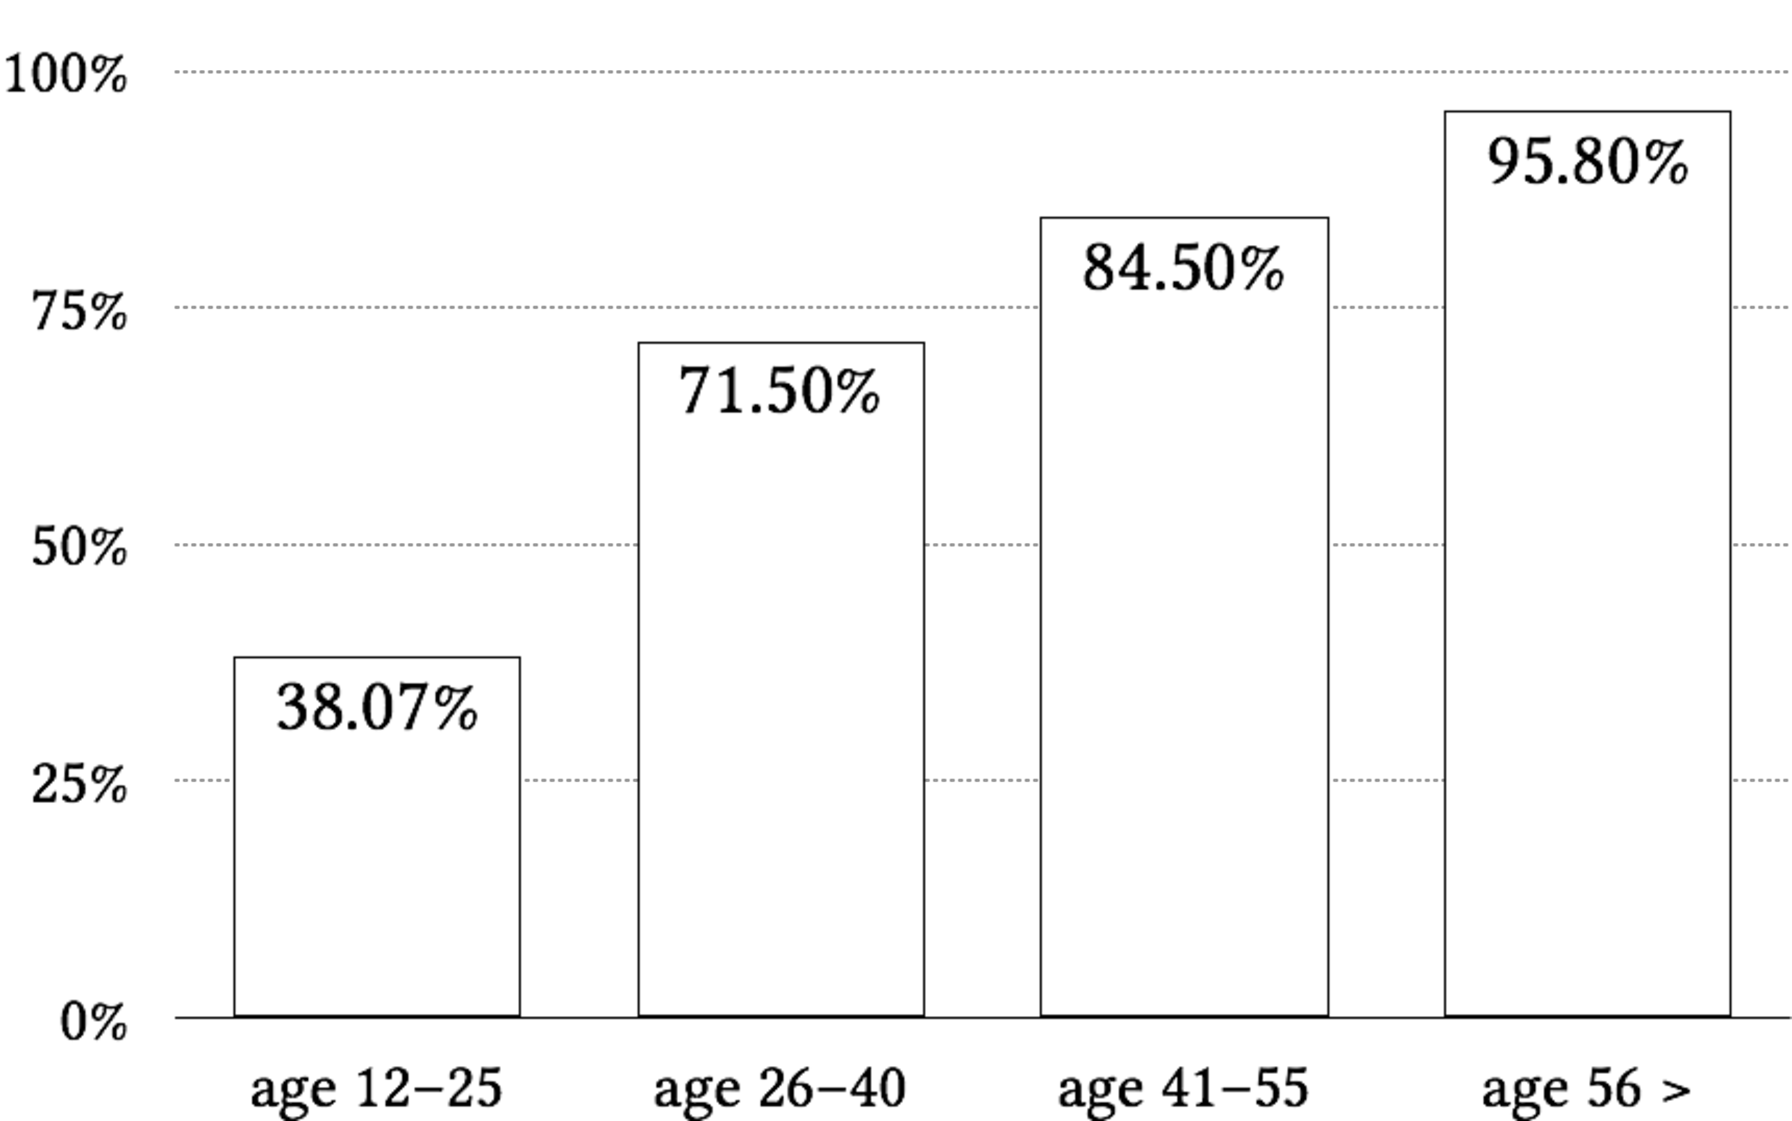
\includegraphics[width=0.7\textwidth]{illustrations/skevin_fig1}
\caption{Venetian loanwords vs. age of informants \citep[175]{skevin_izmedu_2012}.}
\label{fig:1}
\end{figure}

The results of the interviews held in 2014 have confirmed the decline in the knowledge and use of the Romance lexical variants. They have shown that 7 interviewed speakers between the ages of 22 and 40 know 61.42\% and use 48.16\%\footnote{Both percentages are relative and used for illustrative purposes only because the complexity of speakers’ answers cannot be simplified and displayed in numbers. Sometimes they would claim that they would use the variant if they’ve seen the object that is no longer in use; sometimes they would say that they would use it only in specific situations or only with other speakers of the Betina dialect. In either of these cases, we would mark their answer as if they had claimed that they use it in all social contexts and situations.} of the words from the questionnaire. The speakers of the Betina dialect in some cases claim to avoid a number of lexical variants, as shown in \tabref{tab:4}. Even though 6 out of 7 speakers know the meaning of words like \textit{bruncin} 'a type of a cooking bowl', \textit{dontrina} ‘religious education’ and \textit{herijada} ‘a small window’, they also say that they would never use them in a conversation with speakers of either their own or of another dialect variety because, according to them, these words are rare or no longer used. For the same reason, they claim not to use words like \textit{kamara }'room' and \textit{kočeta} 'bed'. This means that these Betina variants have already been replaced by SC or SRDD variants. As far as the variants \textit{gučica }‘undershirt’, \textit{intimela} 'pillowcase', and \textit{trkulati} ‘to produce olive oil’ are concerned, they would use them only in conversations with speakers from Betina. This means that, over time, these variants are also likely to be replaced by SRDD or SC expressions. 

\begin{table}
\resizebox{\textwidth}{!}{
\begin{tabular}{lp{.3\textwidth}p{.3\textwidth}p{.2\textwidth}p{.2\textwidth}}
\lsptoprule

{\bfseries Betina lexical variant} & {\bfseries No. of informants of the seven interviewed who know the meaning} & {\bfseries No. of informants of the seven interviewed who claim to use the word} &  & \\
\\
\multicolumn{3}{p{\textwidth}}{{\bfseries Variants that have already been replaced by an SRDD or SC variant}} & {\bfseries SRDD variant} & {\bfseries SC variant}\\
\midrule
{\bfseries \textit{bruncin} 'a type of cooking bowl’} & 6 & 0 & {\itshape {}-} & {\itshape lonac}\\
{\bfseries \textit{dontrina} ‘religious education’} & 6 & 0 & {\itshape {}-} & {\itshape vjeronauk}\\
{\bfseries \textit{herijada} ‘a small window’} & 6 & 0 & {\itshape ponistr(ic)a} & {\itshape {}-}\\
{\bfseries \textit{kamara} 'a room‘} & 7 & 0 & {\itshape {}-} & {\itshape soba}\\
{\bfseries \textit{kočeta} 'a bed‘} & 7 & 0 & {\itshape posteja} & {}-\\
\\
\multicolumn{3}{p{\textwidth}}{{\bfseries Variants that the speakers use only in conversations with speakers of the Betina dialect. In conversations with other speakers they use either the SRDD or the SC variant:}} & \textbf{SRDD variant} & \textbf{SC variant}\\
\midrule
{\bfseries \textit{gučica }‘an undershirt’} & 7 & 7 & {\itshape kanotijera} & {\itshape potkošulja}\\
{\bfseries \textit{intimela}  'a pillowcase'} & 7 & 7 & {\itshape {}-} & {\itshape jastučnica}\\
{\bfseries \textit{trkulati }‘to produce olive oil’} & 7 & 7 & {\itshape napraviti ulje; (u)činiti uje} & {\itshape {}-}\\
\lspbottomrule
\end{tabular}
}
\label{tab:4}
\caption{Examples of intrasystemic quantitative reduction as a consequence of a convergence toward SRDD and toward SC.}
\end{table}

On the other hand, there are variants (which are listed in \tabref{tab:5}) that can also be considered salient because they are used only in the Betina dialect (e.g., \textit{lohunara/lehunara}) or only in the varieties of the island of Murter (e.g., \textit{bublija}). Still, the speakers claim that they use them in communication with speakers of other varieties. It is unlikely that the speakers are not aware of their markedness, so we can presume that, for some reason, these variants signal the speaker’s identity as a member of a group \citep[85]{chambers_dialectology_2004}.

\begin{table}
\resizebox{\textwidth}{!}{
\begin{tabular}{p{.15\textwidth}p{.4\textwidth}p{.3\textwidth}p{.3\textwidth}}
\lsptoprule
{\bfseries Betina lexical variant} & {\bfseries meaning} & {\bfseries No. of informants of the seven interviewed who know the meaning} & {\bfseries No. of informants of the seven interviewed who claim to use the word with speakers of their own and of other varieties}\\
\midrule
{\bfseries\itshape lehunara/ lohunara} & 'a type of a small fishing net in the form of sack on a long stick' & 6 & 6\\
%{\bfseries\itshape bublȉja} 
& 'a round Easter cake, a type of sweet bread' & 7 & 7\\
{\bfseries\itshape čikara} & 'a mug' & 7 & 7\\
{\bfseries\itshape loštijera} & 'a baking tray' & 7 & 7\\
{\bfseries\itshape prsura} & 'a frying pan' & 7 & 7\\
{\bfseries\itshape škabelin} & 'a nightstand' & 7 & 7\\
\lspbottomrule
\end{tabular}
}
\caption{Examples of divergence}
\label{tab:5}
\end{table}

\section{ Semiotic space as the space of identity}
Objects that seem to be merely utilitarian are often part of a particular space; they signify and issue messages about the society’s priorities, ways of life, culture, and traditions (see \citealt[110]{hawkes_structuralism_2004}). Each utilitarian object, such as \textit{brganja, lohunara, hildošpanja, karutula }and \textit{pot }acknowledges the way people used to organize their lives and the way they structured their social and cultural identity. \textit{Brganja, lohunara }and\textit{ hildošpanja }issue presuppositions concerning inhabitants’ adherence to fishing and to the sea.\textit{ Karutula,} a type of braided cake’ was traditionally prepared for children at Easter. As an additional gift, one whole egg would be baked inside the cake on the bottom end of the cake. Also, \textit{pot }is not merely ‘a metal container with a handle’ out of which people used to drink, but the manifestation of a custom to make \textit{bevanda }(red wine with water) and to pass it around the table so that everyone could drink out of the same \textit{pot. }The meaning of an object is largely attached to its function, its utility in relation to the repertoire of human needs \citep[48]{moles_theorie_1972}; that is, as soon as there is a society, every usage is converted into a sign of itself \citep[41]{barthes_elements_1968}. In this work we use the Lotmanian term of semiotic space to refer to all aspects of human existence and to stress that external factors, such as culture, society, fishing, wooden boat building, and ways of earning money or getting food, can acquire semiotic meaning. In Lotman’s words, they influence the consciousness of man only when they have corresponding signifiers to name them because “for human thought all that exists is that which falls into any of its languages” \citep[134]{lotman_culture_2009}. This means that, even if some social or cultural aspects of Betina still exist, if the speakers don’t know the signifiers to name these aspects, it is as if they did not exist, which means that the local identity and distinctiveness are lost to their thought. It also works the other way around: if the cultural and social aspects are lost, it won’t take long for the signifier, emptied of its signified, to be lost as well.

\section{Changes in semiotic space \textit{vs.} the reduction of intrasystemic variation}
In the case of dialect levelling caused by the linguistic accommodation of speakers, the replacement of dialect variants with SRDD or SC variants occurs. In the case of dialect levelling caused by changes in the semiotic space, no such replacement occurs because the object or a human practice that has been lost doesn’t need a new signifier. Nonetheless, dialect levelling still occurs because there is a reduction in intrasystemic variation, which leads to simplification, homogenization and the levelling of a dialect variety and of its cultural and local distinctiveness, making it more similar to a supra-regional or standard variety.

Changes in semiotic space are parallel to changes in human needs and praxis, and can be analysed from three standpoints: 

\begin{enumerate}
\item the complete disappearance of utilitarian objects that used to be very effective sociocultural signs 
\item the loss of an object's utilitarian and functional importance in everday life
\item the transfer of such an object from one semiotic space to another.
\end{enumerate}

These are three hypothetical reasons that supposedly cause the loss of intrasystemic quantitative variation as a consequence of change in a semiotic space. To illustrate these points and to show our interest in the cognitive effect on the interpreter, the variants and their referents are represented through Peirce's semiotic triangle. The semiotic triangle begins with an understanding of the sign as the primary element of any semiotic system. Strictly speaking, semiosis, and not the sign, is the proper object of semiotic study. The realization of a semiological sign in a communication process depends on the interlocutors, on the objects, and on the context in which the communication occurs. In this case, the analysis of the communication process is relevant both to the addresser and to the addressee. 

\subsection{The disappearance of utilitarian objects}
It is common knowledge that very often a word survives even though the object it represents has disappeared, which is the case with the word \textit{dumplir}. All of the older speakers who participated in the 2008, 2009 and 2010 interviews knew its meaning, while only one of the young speakers was familiar with its meaning.

\begin{figure}
\begin{tabular}{ccc}
\lsptoprule
{\bfseries Older speakers} & {\bfseries Young adults} &
\begin{minipage}[t]{0.3\textwidth}{\bfseries Loss of the lexical variant}\end{minipage}\\
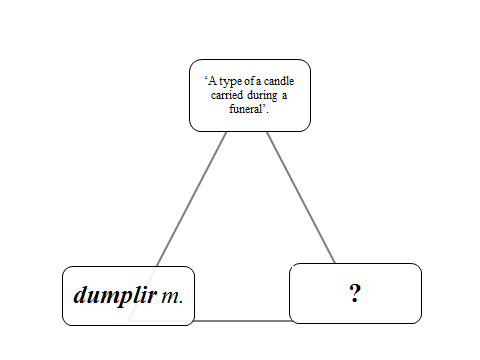
\includegraphics[width=0.3\textwidth]{illustrations/skevin_fig21} &
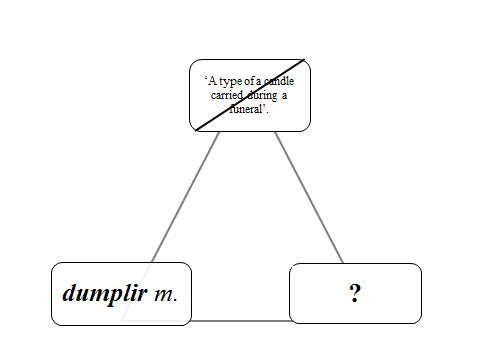
\includegraphics[width=0.3\textwidth]{illustrations/skevin_fig22} &
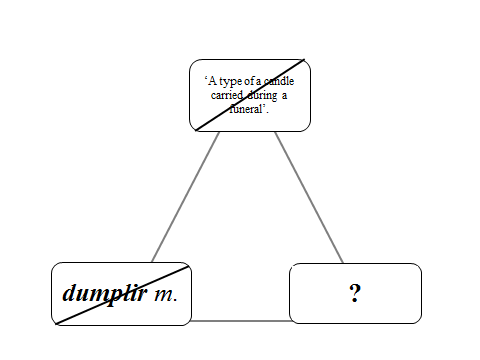
\includegraphics[width=0.3\textwidth]{illustrations/skevin_fig23}\\
\begin{minipage}[t]{0.3\textwidth}{\bfseries \textit{Dumplir}, which means `a wooden candlestick carried during a funeral,' is not in use anymore, although the older speakers still have a mental picture of it in their minds and are able to describe it.}\end{minipage} & 
\begin{minipage}[t]{0.3\textwidth}Over time, there will not be any speakers who  can decribe it (unless it has been described in some written text such as a dialectal glossary).\end{minipage} & 
\begin{minipage}[t]{0.3\textwidth}When an object has disappeared, the addresser and the addressee cannot communicate, the object as a semiological sign cannot have any cognitive effect on the addressee, and it is no longer possible to close the circle of semiosis by finding exclusively the same interpretant at both ends of the communication process. Meaning without communication is not possible, so, over time, the word disappears as well.\end{minipage}\\
\lspbottomrule
\end{tabular}
\label{fig:2}
\caption{Loss of intrasystemic quantitative variation.}
\end{figure}


\subsection{The loss of an object’s utilitarian and functional importance in everyday life}
\tabref{tab:1} shows that the traditional wooden boat building sector decreased by 12\% in the period from 1971 to 2001. The same happened to agriculture and fishing, which in the same period decreased by 17\%. These trends lead to a loss of importance in these human practices and consequently of the utilitarian objects affiliated with them. They also affect the general familiarity of speakers with other topics of conversation, such as the weather, the winds, the behaviour of the sea, the points of the compass, fishing tools, boat-building tools, and boat parts. Consequently, they also affect the speakers’ recognition and awareness of the signifiers. For example, young speakers know the terms for some of the most prominent parts of a traditional boat (e.g.,  \textit{prova} 'bow' or \textit{pajoli} 'wooden floor of a boat'), but they are uncertain when asked about less prominent and smaller parts, such as \textit{mankul }'a thick wooden post around which a mooring rope is tied' or \textit{maškul, soha }or\textit{štiva}. In the case of \textit{mankul}, 3 out of the 7 speakers interviewed guessed that it was something on a boat but could not identify the exact referent. Why should they know these words? someone might ask. Because they used to be, and on paper still are, signs that create the semiotic space of Betina, whereas today they belong to very specialized semiotic spaces whose language is accessible only by those who work in that field. Just as people live nowadays with their tablets, computers, and smart-phones, people in Betina, only a few decades ago, used to live with the sea and their boats. This is in fact what Lotman refers to as a secondary modeling system interwined with a primary modeling system, that is, with a natural language. The different substructures of the semiosphere are linked in their interaction and cannot function without the support of each other. \citep[219]{lotman_semiosphere_1985}.

\begin{figure}
\begin{tabular}{cc}
\lsptoprule
{\bfseries Older speakers} & {\bfseries Young adults}\\
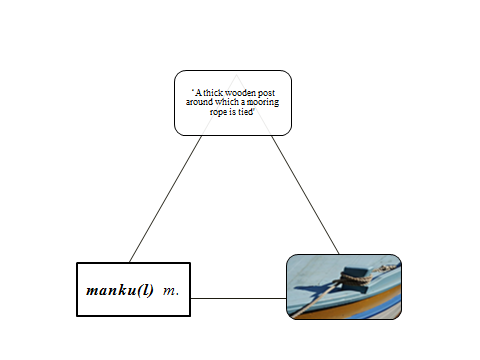
\includegraphics[width=0.4\textwidth]{illustrations/skevin_fig31} & 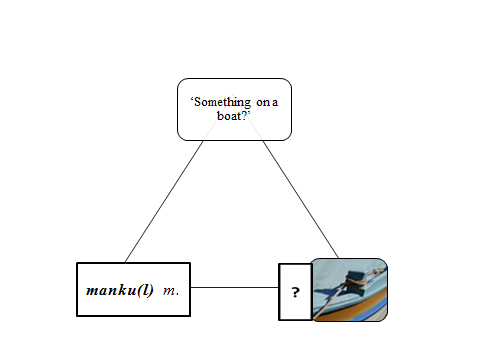
\includegraphics[width=0.4\textwidth]{illustrations/skevin_fig32}\\
\begin{minipage}[t]{0.4\textwidth}{\bfseries Older speakers can identify without any problem the referent as  `a thick wooden post around which a mooring rope is tied'.}\end{minipage} & 
\begin{minipage}[t]{0.4\textwidth}Young speakers suppose that it is something on a boat, but cannot identify the referent.\end{minipage}\\
\lspbottomrule
\end{tabular}
\caption{Restriction of the number of users.}
\label{fig:3}
\end{figure}

\begin{figure}

\includegraphics[width=0.5\textwidth]{illustrations/skevin_fig3_mankul}
\label{fig3_mankul}
\caption{A \textit{mankul}.}
\end{figure}


This analysis has shown that speakers know 53.05\% of the words that name objects and concepts that have lost importance in everyday life in Betina. This means that there is still some adherence to the traditional and that the identity of Betina is still recognized in some traditional crafts, although the average speaker’s knowledge of words does not always keep pace with this identity projection. To this list belong the names of parts of the National costume (\textit{bušt, ogrica}), parts of some fishing tools (\textit{hildošpanja/fildošpanja}), fish parts (\textit{lustra, butarga}), or the names of the winds and sea storms (\textit{brganjaš, baraškada, šijun). }There are also variants whose meanings are more well known, which can be explained by the fact that they also belong to the lexis of SRDD (e.g., \textit{trmuntana/tremuntana}) or by their semantic transparency (e.g., \textit{kamenica, mastač}). 

\subsection{The transfer of an object from one semiotic space to another}
\subsubsection{The resemantization and refunctionalization of traditional utilitarian objects}

\textit{Brganja} is a Venetian loanword \textit{par excellence}. To this day, it has always had a very imporant role in the everyday life of Betina. The fact that, through the centuries, new words were formed by adding Croatian endings to the original Venetian form \textit{bragagna} testifies to the importance of its uses in the past. For example, the verb \textit{brganjati, }meaning to collect sea shells with this tool', or the name of the wind \textit{brganjaš, }which favors bottom trawling with a \textit{brganja}. With the birth and development of tourism, a new expression, \textit{Dan Brganje (Brganja Day}) has also been coined. This is the name of a festival celebrated in Betina every summer on the first Sunday of August. Today, the use of this fishing tool is forbidden. Still, \textit{brganja} is one of the most vital fishing terms in Betina, and all of the interviewed speakers knew the word. 

\begin{figure}
\begin{tabular}{ccc}
\lsptoprule
{\bfseries Older speakers} & \multicolumn{2}{l}{{\bfseries Young adults: semantic extension}}\\
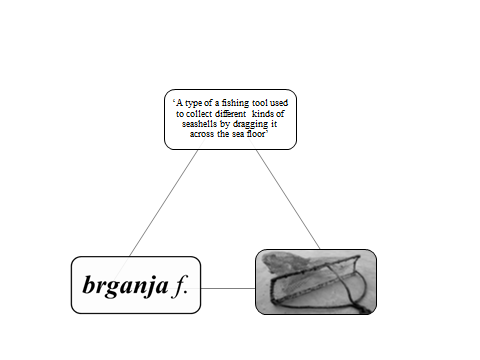
\includegraphics[width=0.3\textwidth]{illustrations/skevin_fig41} &
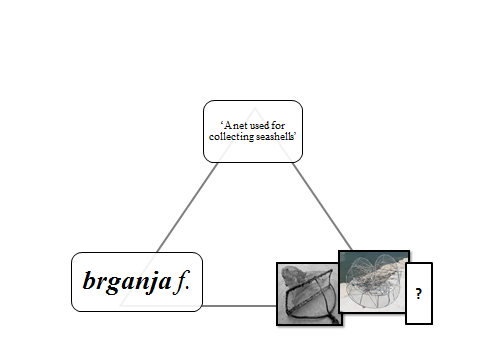
\includegraphics[width=0.3\textwidth]{illustrations/skevin_fig42} &
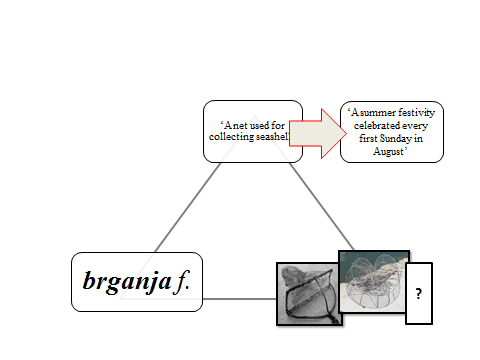
\includegraphics[width=0.3\textwidth]{illustrations/skevin_fig43}\\
\begin{minipage}[t]{0.3\textwidth}{\bfseries This is a triadic relation formed in the mind of an older speaker but not in the minds of the young informants. This word has a different effect on young speakers.}\end{minipage} & 
\begin{minipage}[t]{0.3\textwidth}This is a triadic relation formed in the mind of a young speaker. The second element of Peirce's semiotic triangle, the \textit{thing signified} or \textit{referential object,} varies. Five out of seven speakers are unsure about the correct referential object; they either describe another fishing tool, or they don't know how to describe it. But all of them, without exception, know its function. Thus, communication is still fulfilled at the pragmatic level.\end{minipage} &
\begin{minipage}[t]{0.3\textwidth}Young speakers know this word thanks to the fact that the community of Betina has refunctionalized it; that is, it has changed its function and accordingly its semiotic space. This word traditionally signified a tool which for centuries was used by the inhabitants of Betina on a daily basis, mostly to get food. A few decades ago, a new substance was attributed to this word: the value of tradition and of collective memory through the name of the festival \textit{Dan Brganje }(Brganja Day).\end{minipage}\\
\lspbottomrule
\end{tabular}
\caption{Change in intrasystemic qualitative variation through resemantization and refunctionalization of the utilitarian objects.}
\label{fig:4}
\end{figure}

\begin{figure}
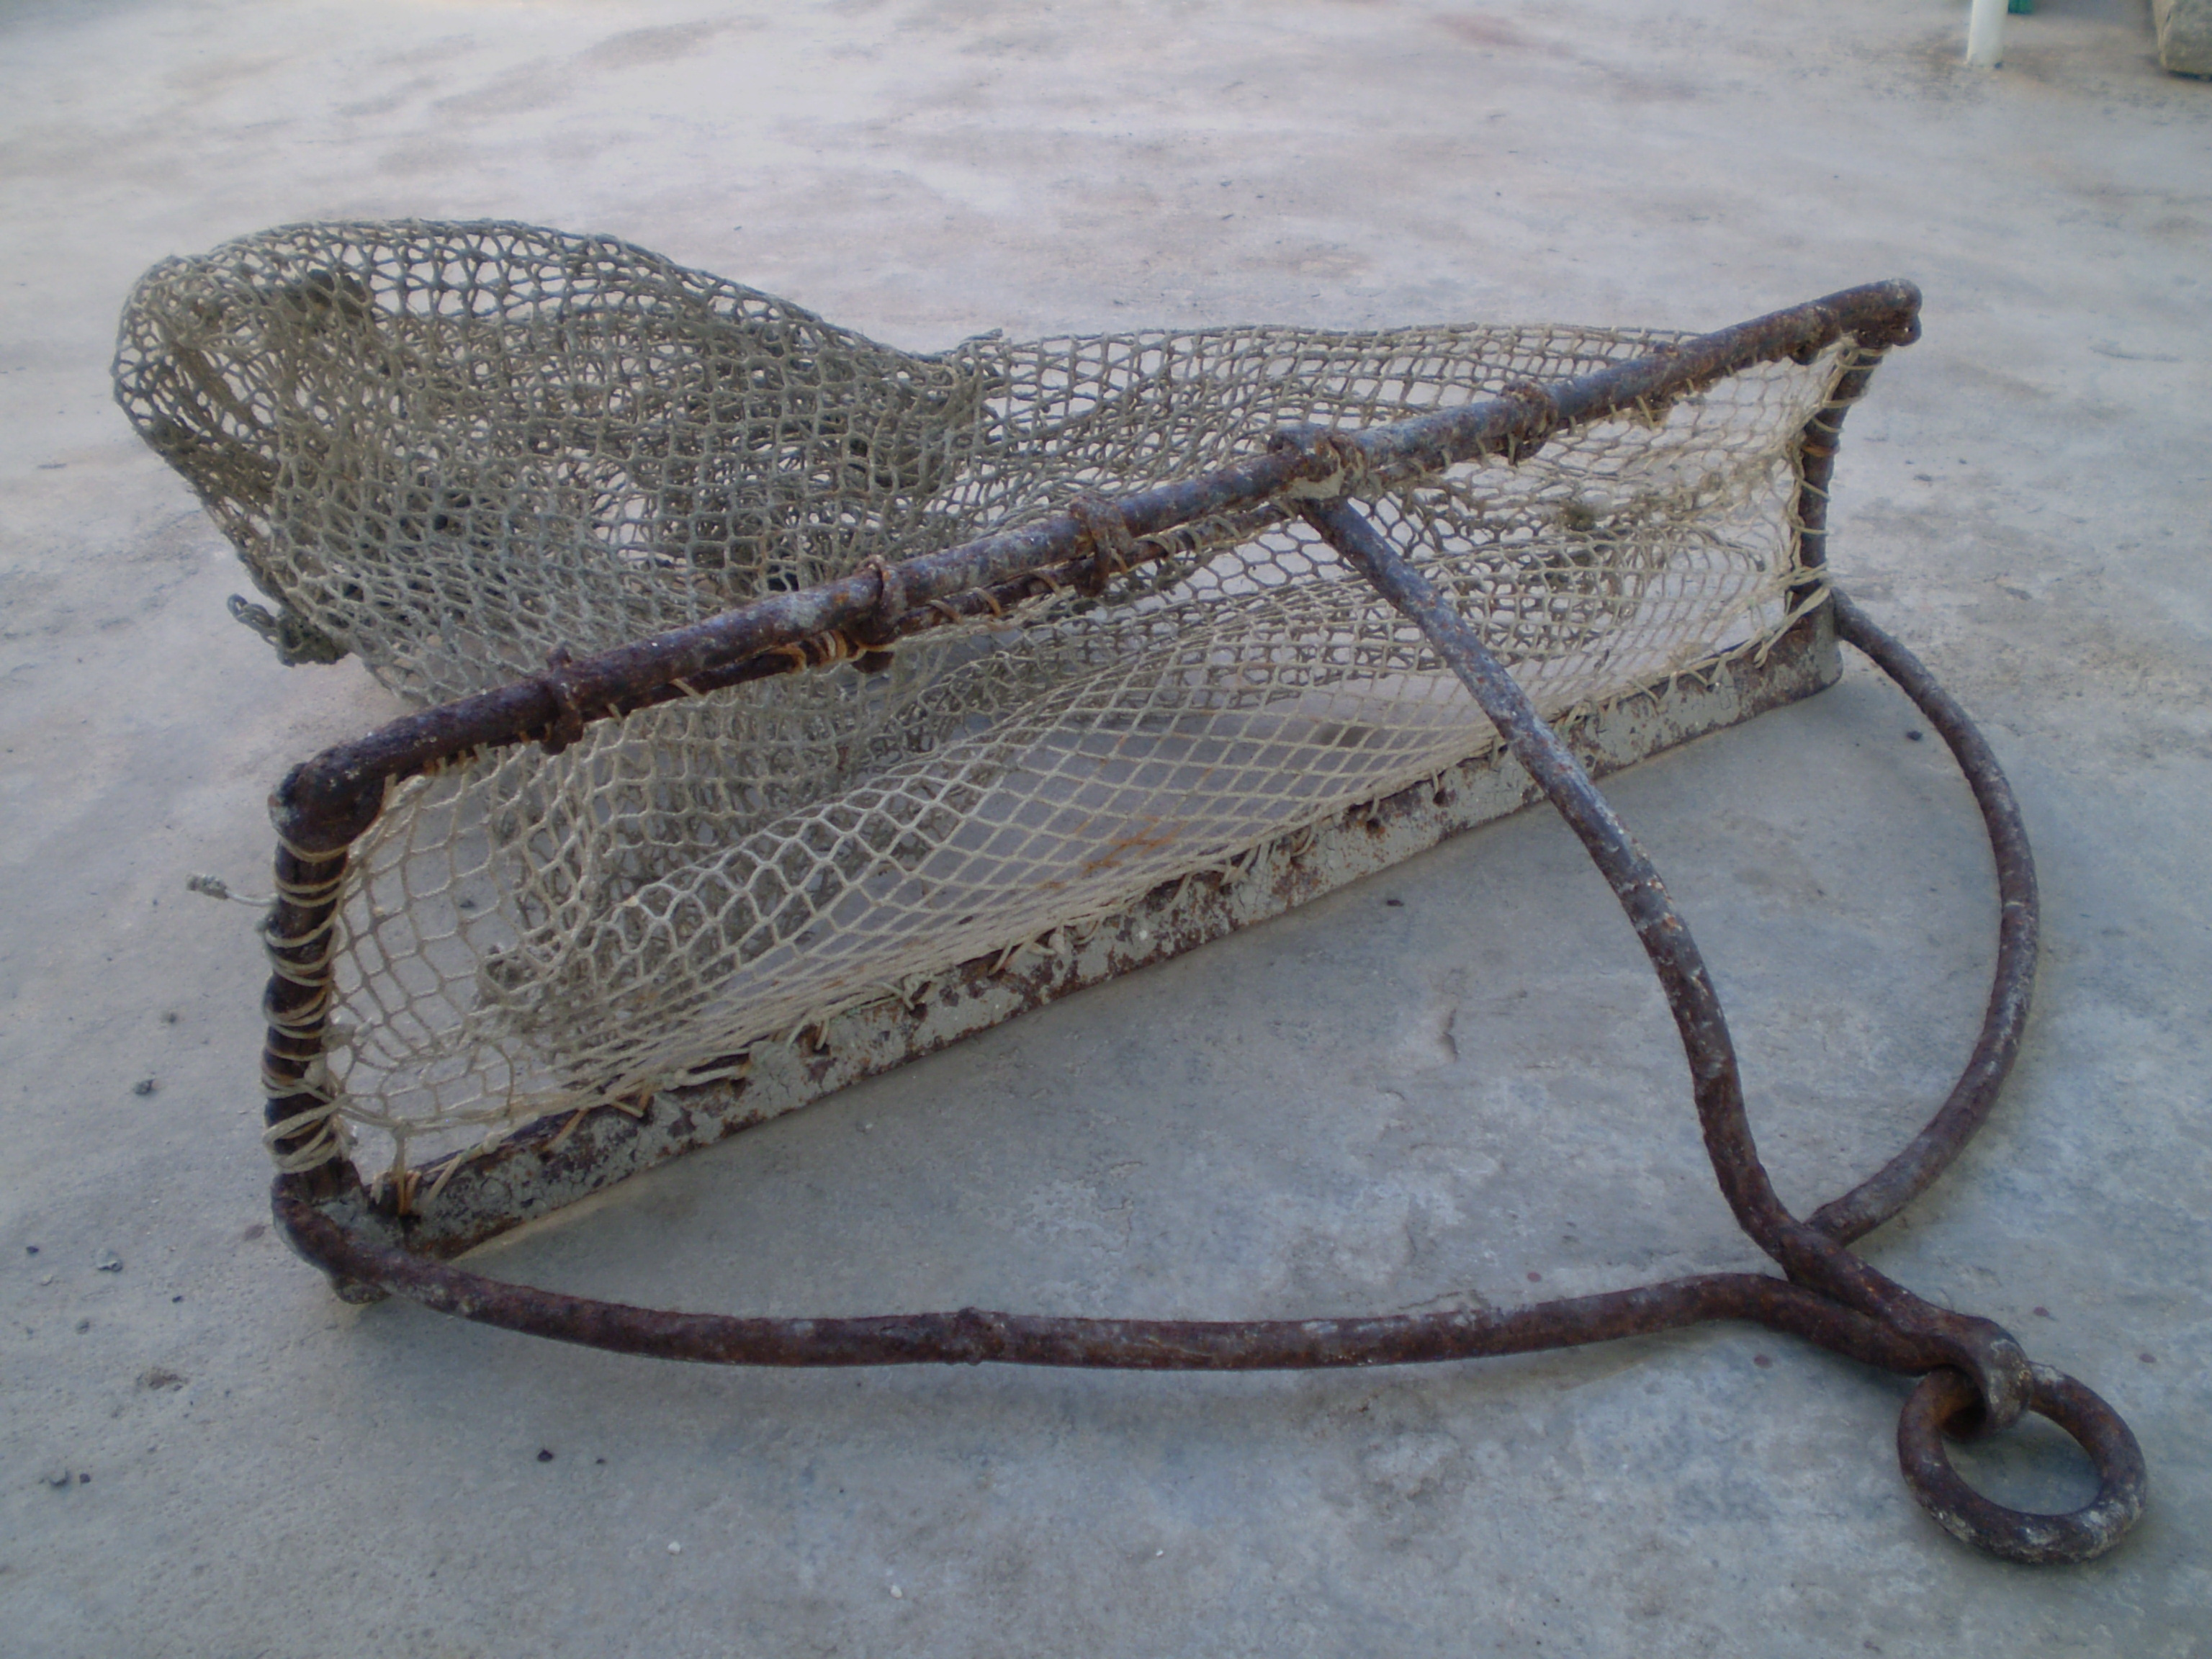
\includegraphics[width=0.45\textwidth]{illustrations/skevin_fig4_brganja}~~~
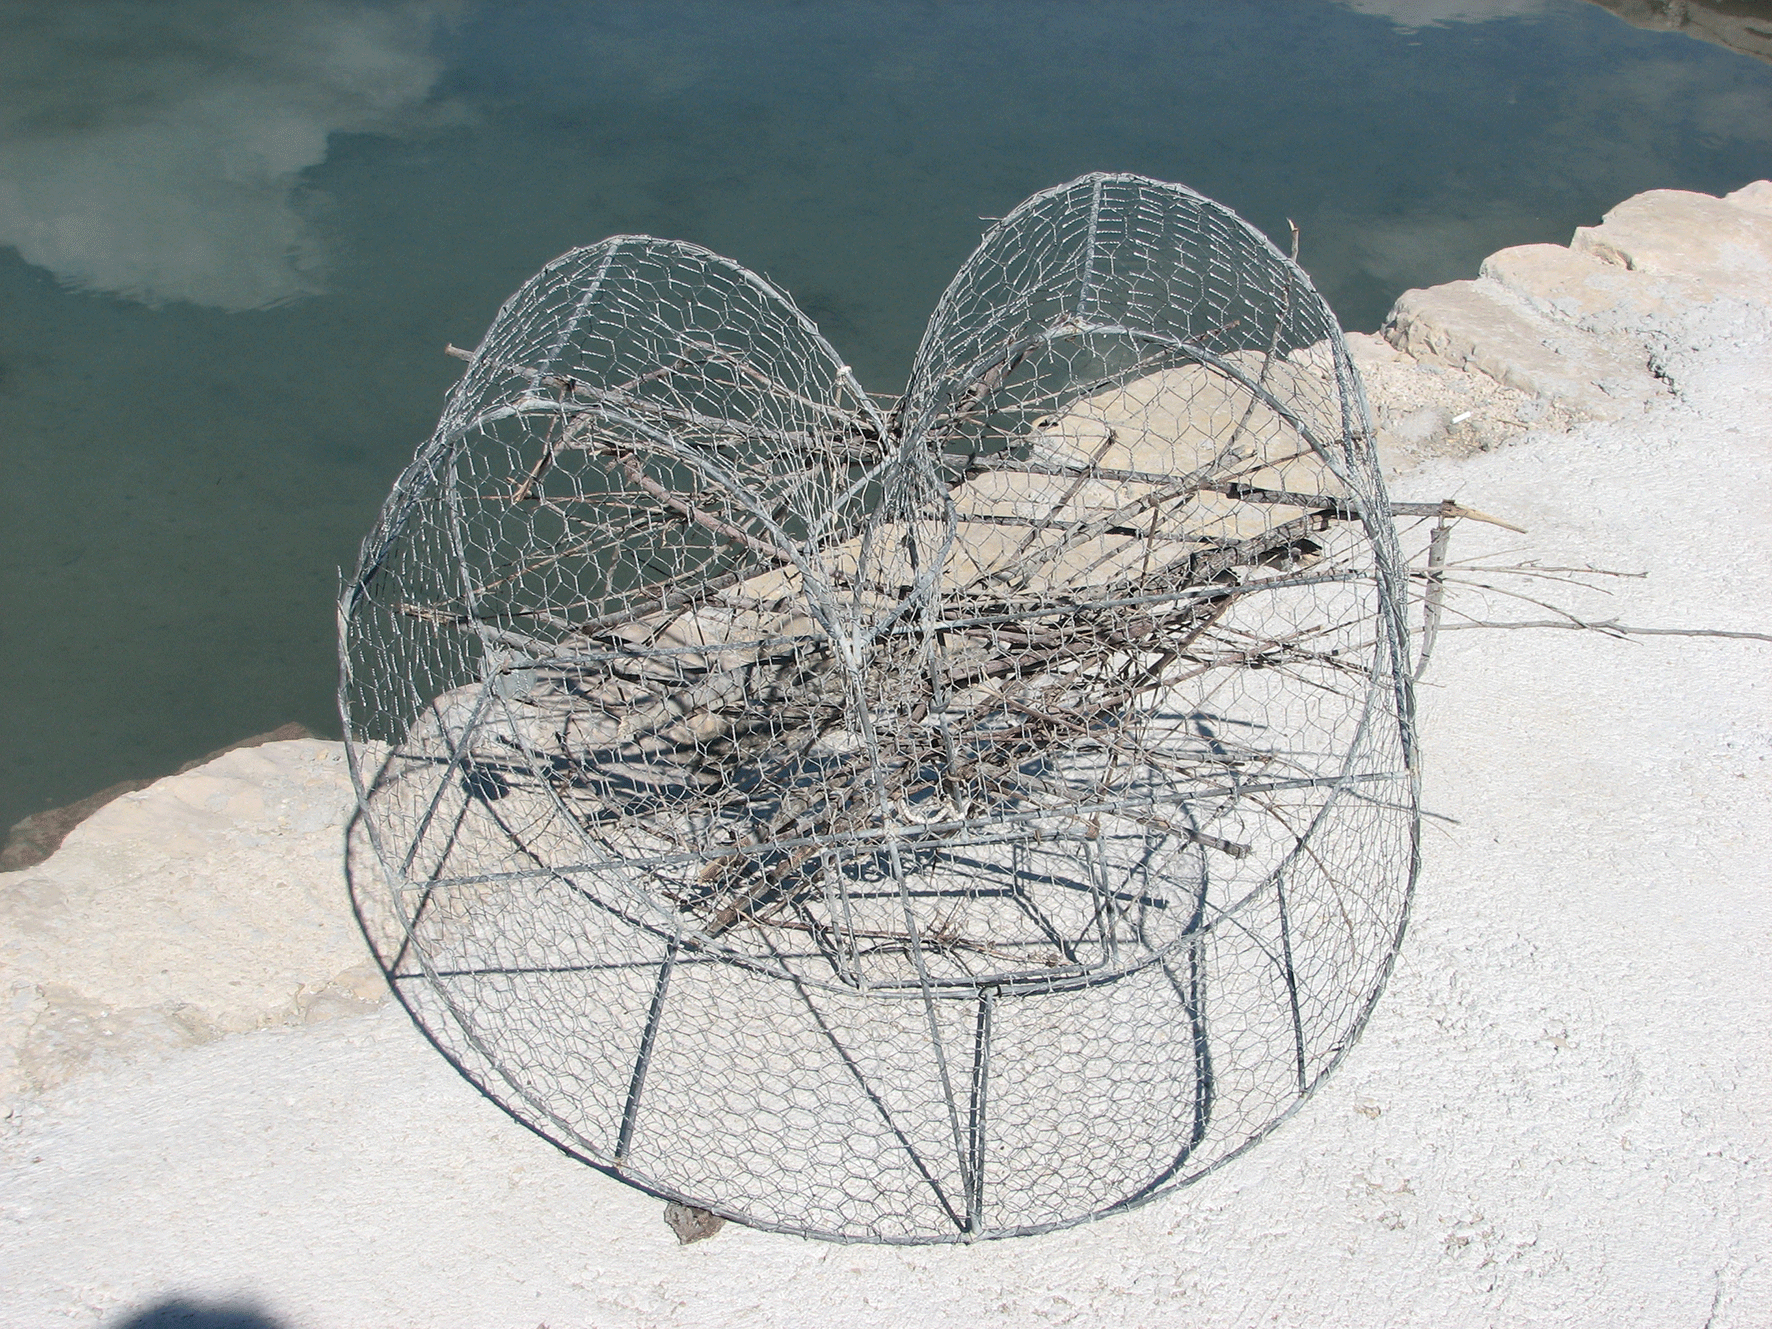
\includegraphics[width=0.45\textwidth]{illustrations/skevin_fig4_vrsa}
\label{fig4_brganja_vrsa}
\caption{A \textit{brganja} (l.) and a \textit{vrša}.}
\end{figure}

This is an example of the extension, or rather, the commercialization of the meaning, since \textit{brganja}, removed from its original semiotic space, that of a fishing tool, has produced a new one, closer to and more appropriate for today’s society and economy, which is oriented mostly toward tourism and no longer toward fishing. Trudgill  explains this phenomenon in the following way: 

\begin{quote}
The remaining variation, i.e. the forms that are not removed during koineisation… will tend to be re-assigned according to certain patterns. This reallocation can cause variants to take on a specialised linguistic (allophonic) or extra-linguistic (social, stylistic, or geographical) function. (1986: 110-126 in \citealt[46]{auer_study_2004})
\end{quote}

There are other examples of semantic extension, such as the variant \textit{škohuni}, which used to refer to a type of shoes, usually made of rubber and rags, worn to work in the field, whereas today, young speakers, besides the original meaning, also know a metaphoric one, i.e., 'cumbersome, usually old and not very elegant shoes'.

\subsubsection{The aestheticisation and refunctionalization of traditional utilitarian objects}

A change in the utilitarian value of the objects, through their aestheticisation and refunctionalisation as decorative items or objects primarily used to re-evoke tradition, can cause a shift in the stylistic meaning of the variants such as in the case of the use of traditional cups and dishes (\textit{pot, potić, pičona, }or \textit{bukara}) or of different kinds of baskets and vessels (\textit{koha}, \textit{konistra,} or \textit{kopanja}). 

\begin{table}
\resizebox{\textwidth}{!}{
\begin{tabular}{lp{.4\textwidth}p{.3\textwidth}p{.3\textwidth}}
\lsptoprule
{\bfseries Lexeme} & {\bfseries meaning} & {\bfseries No. of informants of the seven interviewed who know the meaning}\ & {\bfseries No. of informants of the seven interviewed who claim to use the word}\\
{\bfseries bukara} & 
`a large wooden wine cup' & 7 & 7\\
{\bfseries pičona} & 
`a metal cup with a handle' & 7 & 7\\
{\bfseries pot, potić} & 
`a smaller metal bowl with a handle' & 6 & 6\\
{\bfseries koha} & 
`a type of a wicker basket, flat and round' & 4 & 4\\
{\bfseries kopanja} & 
`a wooden vessel used for kneading dough' & 2 & 2\\
\lspbottomrule
\end{tabular}
}
\caption{The aestheticisation and refunctionalization of objects}
\label{tab:6}
\end{table}

The refunctionalization of the objects listed in \tabref{tab:6} consists in using them as decorative or even utilitarian items in traditional restaurants, hotels, and houses for rent. Their purpose is to re-evoke tradition and old customs such as kneading dough in a \textit{kopanja }or serving wine in a \textit{bukara}. They still serve a purpose by means of their traditional utilitarian function being switched to a new aesthetic function: to attract tourists in a changed context and in a changed economy that today relies on tourism up to 45\% (as illustrated in \tabref{tab:1}). Thanks to these processes, some of the variants, like \textit{bukara, pot,} and \textit{pičona}, by taking on a new social and stylistic function, are better known to the speakers. 

\section{Conclusions}
This study has confirmed that young speakers, when talking about familiar and everyday subjects, converge in their communication with speakers of other dialect varieties by eliminating salient lexical variants that they consider rare or “out of use” (\textit{kamara, kočeta}). On the other hand, it has also shown that the informants diverge from their interlocutors by using lexical variants typical of island varieties (\textit{bublija}) or\textit{ }of the Betina variety in particular (\textit{lehunara/lohunara}). This indicates that young adults still want to be identified with their speech community and recognized as members of that group of speakers. 

The study has also confirmed that a change in semiotic space can lead to quantitative or qualitative intrasystemic variation or to a reduction of the number of users. 

A complete disappearance of objects causes a reduction in intrasystemic quantitative variation, i.e., a loss of lexical variants, which leads to cultural and dialect levelling. Therefore, a loss of referents will over time cause a loss of local variants such as \textit{bujo(l), dumplir, murtar, taraban, }and \textit{škapular. }

There are cases in which, due to the object’s refunctionalization, resemantization, or aestheticisation, no such loss occurs. It has proven that the transfer of objects from one semiotic space to another, when an object gets refunctionalized, leads only to semantic change because of the extension of the meaning of the variants (\textit{brganja, škohuni}). However, only a very small number of lexical variants belong to this group. If refunctionalization and resemantization does not occur, over time this will lead to a reduction of intrasystemic lexical variation, as well as cultural and dialect levelling. 

The analysis shows that speakers know the meanings of 53.05\% of the words referring to objects and concepts that still exist but have lost their utilitarian and functional importance in everday life (e.g., \textit{mankul, butarga, šijun, fildošpanja/hildošpanja, burtižati}). Since these words have ceased to be important to the wider speech community, this implies a restriction in the number of users and consequently, a loss of cultural and dialect diversity as well as cultural and dialect levelling.

Since the interviews and the analysis have shown that young adults in Betina converge and diverge in more or less the same number of situations and variants, this research has shown that changes in semiotic space (at least in the case of Betina) are in fact the most prominent reason for dialect levelling. 

Naturally, with this change of approach we do not claim to have found all the reasons for dialect levelling. We just claim that this is another possible approach to understanding this phenomenon. On the contrary, in our corpora there are some lexical variants whose status in the lexis of the Betina dialect cannot be explained by means of any of the proposed approaches (i.e., the saliency factor, linguistic accommodation, or the loss of utilitarian objects and human praxis). For example, we could not find a valid answer to why the variant \textit{gvantijera, }which refers to such an ordinary and everyday object as a tray is almost lost to the knowledge and usage of the young adults (3 out of 7 speakers know its meaning, but none of them uses the word), whereas \textit{kajin }‘a round metal vessel used for washing clothes’\textit{, }a household object as well, but no longer in use, is very familiar to all the speakers, and all of them claim that they would use the word if they saw the object. This and many other questions on the future of dialects have yet to be answered and can be explained neither through the semiotic nor through the sociolinguistic approach.

\printbibliography[heading=subbibliography,notkeyword=this]
\end{document}